\begin{figure}[h]
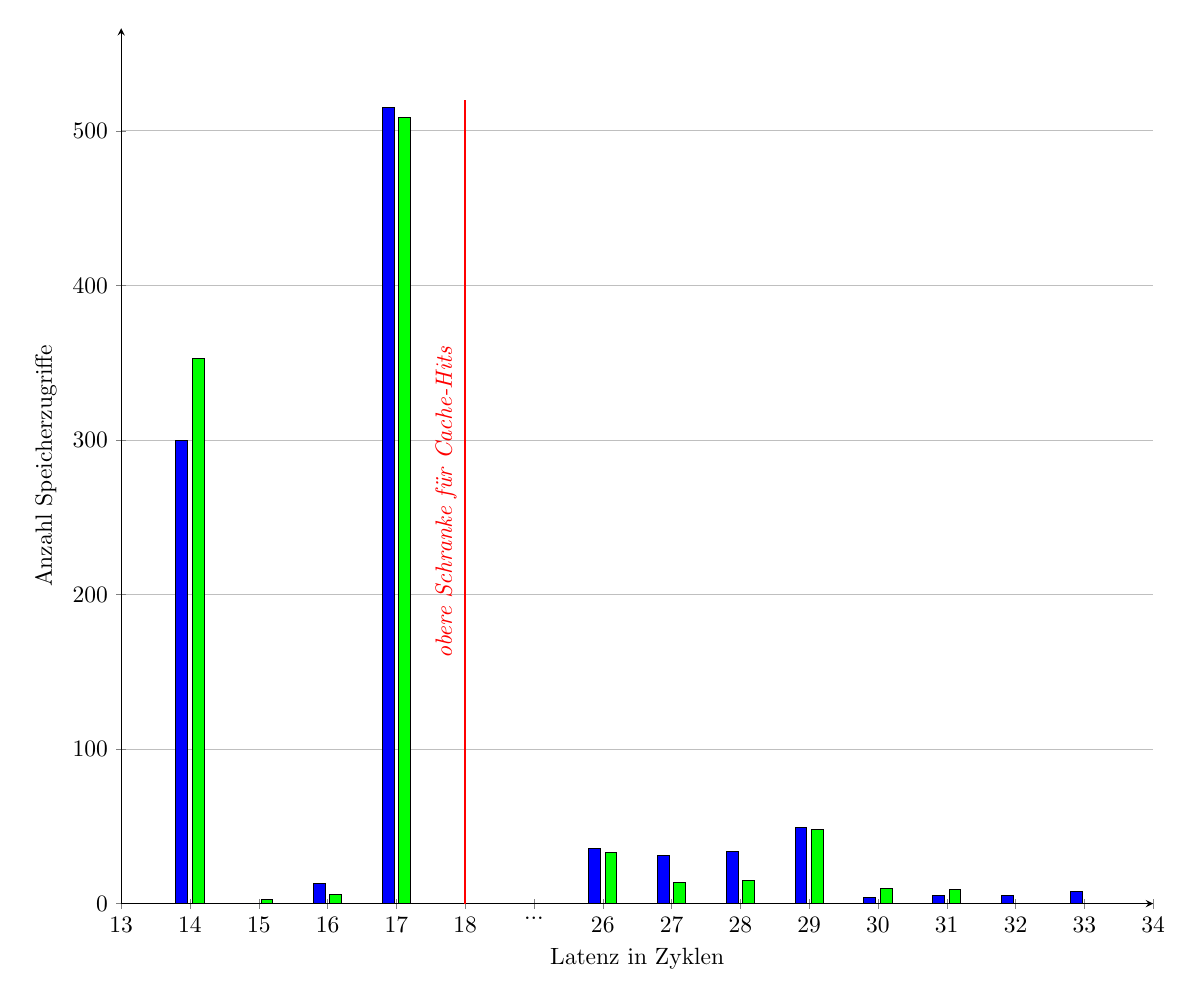
\begin{tikzpicture}[scale=0.85]
 
  \begin{axis}[
    width=17cm,
    ybar,
    bar width=5pt,
    point meta=rawy,
    %
    axis x line=bottom,
    axis y line=left,
    ymajorgrids=true,
    %
    ylabel=Anzahl Speicherzugriffe,
    ymin=0,
    ytick={0,100,200,300,400,500},
    enlargelimits=auto,
    %
    xlabel= Latenz in Zyklen,
    symbolic x coords ={$13$,$14$,$15$,$16$,$17$,$18$,...,$26$,$27$,$28$,$29$,$30$,$31$,$32$,$33$,$34$},
    x tick label style={below},
    xmin=$13$,
    xmax=$34$
    ]

    \addplot[fill=blue] coordinates {
      ($14$,300)
      ($15$,0)
      ($16$,13)
      ($17$,515)
      
      ($26$,36)
      ($27$,31)
      ($28$,34)
      ($29$,49)
      ($30$,4)
      ($31$,5)
      ($32$,5)
      ($33$,8)
    };
    
    \addplot[fill=green] coordinates {
      ($14$,353)
      ($15$,3)
      ($16$,6)
      ($17$,509)
      
      ($26$,33)
      ($27$,14)
      ($28$,15)
      ($29$,48)
      ($30$,10)
      ($31$,9)
    };
    
    \draw [thick, red] (axis cs:$18$,0) -- node[above, rotate=90]{\textit{obere Schranke für Cache-Hits}} (axis cs:$18$,520);

  \end{axis}

\end{tikzpicture}
\caption{Anzahl Zugriffe verschiedener Latenzen für die Sequenz \textcolor{blue}{$O_{S,1}$} und \textcolor{green}{$O_{S,2}$}}
\end{figure}
